% Drawing 81/01-5 -- folder 81, batch 01, archive page 10 (PDF page 11).
% Transcription: au bas de la feuille, trois croquis à main levée : à gauche un polygone à six côtés dont deux côtés consécutifs, en bas, sont repassés d'un trait épais, avec à son angle inférieur gauche un petit cercle et un enchevêtrement de traits fins ; au milieu une ligne brisée épaisse en « V » ouvert, doublée de traits fins ; à droite une ellipse traversée de six courbes à peu près verticales.
% Kind: three free-hand sketches: polygon with heavy sides, heavy broken line, ellipse crossed by curves. Method 2 (schematic redraw from the facsimile). Status: ok.
% Notes: Three free-hand ink sketches at the foot of the sheet. Left: a six-sided polygon; its two lower sides are heavy and meet at one vertex, the upper right corner and the lower part of the right side are gone over heavily; at its lower left corner a small circle and thin strokes (two long obliques, a thin triangle below, a curve). Middle: a heavy broken line of two segments, continued by a lighter third rising to the right, and thin strokes doubling it (two from its left end, two falling from its right end). Right: an ellipse crossed by six roughly vertical curves, ends on or near the outline, and a thin stroke from the broken line to the ellipse. Left out: nothing struck. Still differs: the thin tangle at the lower left of the polygon is a reading of overlapping strokes; the curves in the ellipse are approximate. The transcription's note (« un polygone et des lignes brisées épaisses, et une ellipse traversée de courbes ») agrees. Redrawn 2026-11-10 (issue 128): to check again. Question settled by a machine pass on the facsimile, 2026-11-12 (page): the tangle at the lower left of the polygon is a knot of thin unlabelled strokes over a small circle, to which no text refers; the redraw keeps the strokes that can be followed, and no other grouping would show a different figure. Not checked by a reader. 2026-11-14, Claude Opus 5.5, overlay check (issue 147): redrawn stroke by stroke on gridded crops of the 400 dpi colour scan (up to 60 px per unit), rasterised from its own coordinates over it and measured (every stroke within 0.4 unit of its ink on average; all ink of the three sketches within 1.5 units of a stroke); not compiled (no TeX in the session). Changed: the circle of radius 4.6 drawn at the lower left corner of the polygon is not on the page and is removed; what reads there as a small circle is a loop formed by a curve that starts above the corner, sweeps left and down past it and runs on, thin, to a blot at the bottom right, and by a short stroke rising across it from the left; above them a small flat loop of two strokes. The tangle is now drawn as it lies: the left side of the polygon running on below the corner, doubled; the heavy lower sides; the thin parallel to the lower left side ending at the junction; the short curved stroke above the junction; the thin triangle under the corner; the line down to the lower corner (with its small hook) and the line from there up to the junction; two thin strokes and a short dash under the junction and the bundle of strokes falling from it; a small hook on the long curve. Middle: the third leg of the broken line is as heavy as the other two; two thin strokes double the second leg from above; a thin stroke runs on from the first leg past the corner; three thin strokes fall from the foot of the third leg. Right: the outline is not an ellipse but a free-hand oval open at its left (gap of about 3 units), and its six crossing curves, with the knot where the first two cross and the small leaf between the fourth and fifth, are redrawn on their ink; the thin stroke from the top of the broken line runs straight across the oval to a heavy end on its bottom. The top side of the polygon is drawn with its gap. Status set to ok.
% Coordinates: 1 unit = 1 mm = 1/100 of the crop width (bbox in page fractions: [0.1, 0.32, 0.62, 0.53]).
% Redrawn by Claude (claude-fable-5-2), issue #128, 2026-11-10; not checked by a human; not compiled (no TeX in the session).
% Checked by Claude (claude-opus-5-5) 2026-11-14 (issue #147): overlaid on the 400 dpi colour facsimile, corrected; not compiled (no TeX in the session). Not checked by a human. Status: ok.
% Rights: reproduces part of the work -- behind RENDER_TRANSCRIPTS, never published by itself.
\documentclass[tikz,border=3pt]{standalone}
\usepackage{amsmath,amssymb}
\usetikzlibrary{patterns,arrows.meta}
\tikzset{pencil/.style={black!45}, struck/.style={black!35}, mpt/.style={circle,draw,inner sep=1.3pt}, pt/.style={circle,fill,inner sep=0.9pt}, opt/.style={circle,draw,fill=white,inner sep=1.1pt}}
\begin{document}
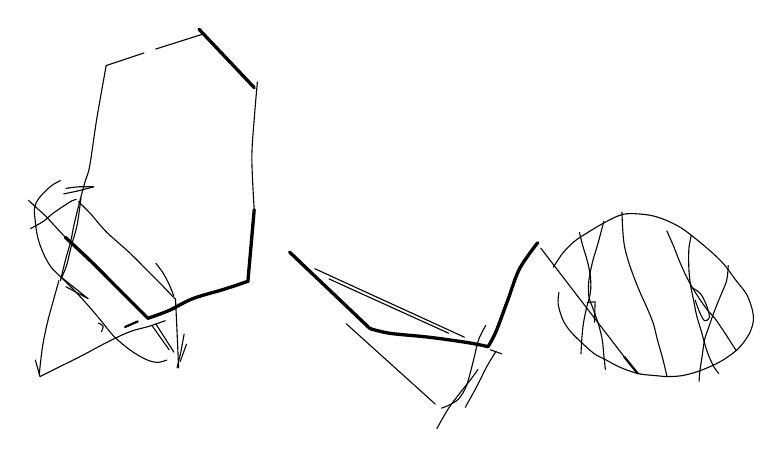
\begin{tikzpicture}[x=1mm,y=1mm,line cap=round,line join=round,font=\scriptsize]
\draw (14,-8.2) -- (18.8,-6.6);
\draw (20.3,-6.1) -- (26.3,-4.2);
\draw[very thick] (25.8,-3.6) -- (32.8,-11);
\draw plot[smooth, tension=0.55] coordinates {(33.2,-10.3) (32.8,-15) (32.5,-20) (32.8,-26.5)};
\draw[very thick] (32.8,-26.5) -- (32,-35.6);
\draw plot[smooth, tension=0.55] coordinates {(14,-8.2) (12.8,-15) (11.9,-21) (11.3,-23) (10.5,-26) (9.9,-28.5) (9.5,-30.5) (8.8,-33) (8.2,-35.5)};
\draw plot[smooth, tension=0.55] coordinates {(10.8,-25) (10.3,-28.5) (9.6,-31) (9,-33.5) (8.4,-35)};
\draw[very thick] plot[smooth, tension=0.55] coordinates {(8.8,-30) (12,-33) (15,-36) (17.5,-38.5) (19.3,-40.3)};
\draw[very thick] plot[smooth, tension=0.55] coordinates {(19.3,-40.3) (22,-39.3) (25,-37.8) (29,-36.6) (32,-35.6)};
\draw (4.1,-25.3) -- (6.3,-27.3) -- (8.8,-30);
\draw plot[smooth, tension=0.55] coordinates {(8.2,-22.8) (7,-23.5) (5.5,-25) (4.9,-26.3) (5,-28) (5.3,-30) (6,-32) (7,-33.8) (8.5,-35.3) (10,-36.8) (12,-39) (13.5,-40.8) (15,-42.6) (17,-44.3) (19,-45.5) (20.5,-45.9) (21.7,-45.6)};
\draw plot[smooth, tension=0.55] coordinates {(4.4,-28.9) (6,-28) (7.2,-27) (8.5,-26.1) (9.6,-25.4) (10.2,-25.2)};
\draw plot[smooth, tension=0.55] coordinates {(8.6,-24.5) (10.5,-24.1) (12.4,-23.6)};
\draw plot[smooth, tension=0.55] coordinates {(8.9,-23.8) (10.5,-23.6) (12.4,-23.6)};
\draw plot[smooth, tension=0.55] coordinates {(10.5,-25.5) (12,-27) (14,-29.3) (17,-32) (19.5,-34.5) (21,-36) (22.7,-37.8)};
\draw (8.2,-35) -- (11.7,-37.8) -- (8.9,-36.3);
\draw plot[smooth, tension=0.55] coordinates {(8,-35.5) (7.3,-38) (6.5,-41) (5.9,-44) (5.5,-47.4)};
\draw (5,-45.6) -- (5.6,-47.7);
\draw plot[smooth, tension=0.55] coordinates {(5.6,-47.7) (8,-46.5) (11,-45) (14,-43.4) (17,-42) (19.5,-41.3) (21.5,-40.6)};
\draw plot[smooth, tension=0.55] coordinates {(13,-40.9) (13.6,-41.3) (13.4,-42)};
\draw[thick] (16.4,-41.4) -- (18,-40.7);
\draw (19.8,-41.2) -- (22,-44.3);
\draw (20.3,-41) -- (22.6,-44.6);
\draw plot[smooth, tension=0.55] coordinates {(20.3,-33.3) (21.2,-34.5) (22,-36) (22.6,-37.5)};
\draw plot[smooth, tension=0.55] coordinates {(22.8,-37.8) (23,-42) (23.2,-46.6)};
\draw (23.9,-42.3) -- (23.5,-44.5) -- (23,-46.6);
\draw (24.2,-43.6) -- (23.4,-45.8);
\draw[very thick] (37.3,-31.9) -- (47.5,-41.6);
\draw[very thick] plot[smooth, tension=0.55] coordinates {(47.5,-41.6) (50,-42.2) (55,-42.7) (60,-43.4) (62.5,-43.9)};
\draw[very thick] plot[smooth, tension=0.55] coordinates {(62.5,-43.9) (63.5,-42) (65,-38) (66.5,-34) (68.8,-30.7)};
\draw (40.5,-34) -- (59.5,-42.7);
\draw (42.3,-35.3) -- (57.5,-42.2);
\draw (44.5,-41) -- (55.8,-51.2);
\draw plot[smooth, tension=0.55] coordinates {(62.2,-41.2) (61.3,-43) (60.8,-45) (60.3,-47) (59.7,-49) (58.8,-50.5) (57.6,-51.3) (56.6,-51.7)};
\draw plot[smooth, tension=0.55] coordinates {(63.5,-44.5) (62.3,-46.5) (61.3,-48.5) (60.5,-50) (59.6,-51.6)};
\draw plot[smooth, tension=0.55] coordinates {(61.2,-46.8) (60.5,-47.8) (59,-49.7) (57.5,-51.7) (56,-54.3)};
\draw (62.8,-44.3) -- (64.2,-44.8);
\draw plot[smooth, tension=0.55] coordinates {(70.8,-33.8) (72,-32) (73.5,-30.5) (75,-29.5) (77,-28.3) (79,-27.3) (80.5,-27) (83,-27.2) (85,-27.8) (87,-28.8) (89,-30.3) (91,-32) (92.5,-33.5) (94,-35.5) (95.3,-37.2) (96,-39) (96.2,-40.5) (95.8,-42) (95,-43.3) (94,-44.4) (92.5,-45.5) (91,-46.3) (89,-47.1) (87,-47.6) (85,-47.7) (84,-47.6) (82,-47.4) (80.5,-47) (79,-46.4) (77.5,-45.6) (76,-44.8) (74.5,-43.5) (73,-42) (72,-40.5) (71.4,-38.5) (71.5,-37)};
\draw (69.2,-31.4) -- (79.8,-45.2);
\draw[thick] (79.8,-45.2) -- (81.5,-47.3);
\draw plot[smooth, tension=0.55] coordinates {(74.1,-29.4) (74.5,-31) (75.1,-33) (75.5,-35) (75.5,-37) (75,-39) (74.6,-41) (74.4,-43) (74.3,-44.8)};
\draw plot[smooth, tension=0.55] coordinates {(77.2,-28) (76.4,-31) (75.8,-33) (75.3,-35.5) (75.3,-37.5) (75.8,-39) (76.5,-41) (77,-43) (77.2,-45) (77.4,-46.8)};
\draw (75.1,-38.3) -- (76.1,-38.2) -- (76,-40.8);
\draw plot[smooth, tension=0.55] coordinates {(79.5,-26.8) (79.6,-29) (79.8,-31) (80.3,-33) (81,-35) (81.8,-37) (82.7,-39) (83.5,-41) (84,-43) (84.7,-45.5) (85.2,-47.6)};
\draw plot[smooth, tension=0.55] coordinates {(85.2,-29.2) (86,-31) (87,-33.5) (88,-35.6) (89.2,-37.6) (90.4,-39.3) (91.3,-40.3) (92.6,-42.2) (94,-44.4)};
\draw plot[smooth, tension=0.55] coordinates {(88.3,-29.8) (88,-31.5) (88,-34) (88.2,-36) (88.6,-38) (89,-40) (89.6,-42) (90,-43.5) (90.5,-45) (91.2,-46.5) (91.8,-47.3)};
\draw plot[smooth, tension=0.55] coordinates {(93,-33.6) (92.8,-35.5) (92,-37.5) (91.2,-39.5) (90.5,-41.5) (90,-43) (89.7,-45) (89.4,-47) (89.3,-48.3)};
\draw plot[smooth, tension=0.55] coordinates {(88.4,-36.4) (89.5,-37.2) (90.3,-38.8) (90.6,-40.2) (90,-40.6) (89.4,-39.6) (88.8,-38)};
\end{tikzpicture}
\end{document}
